
\chapter{Analisi del contesto aziendale}
\section{Vision Lab Apps e il suo ambito di attività}
  Vision Lab Apps S.R.L è una startup nata a New York nel 2011, con sede operativa a Torri di Quartesolo (VI), impegnata nel fornire servizi per la crescita del business delle \nameref{PMI}.
  I prodotti principalmente sviluppati dall'azienda sono \textit{software} personalizzati, siti web per il settore sanitario, manifatturiero e della sicurezza.\\
  È impegnata anche nello sviluppo di servizi \textit{cloud} e \textit{software} per dispositivi \nameref{Wear} e \nameref{IoT} in modo da permettere ai loro utenti di integrarsi in modo migliore con la rete di informazioni e sensori da cui sono circondati nella quotidianità.\\
  In particolare stanno eseguendo ricerca e sviluppo nel campo di visori per la realtà aumentata in modo da supportare le attività lavorative, promettendo grandi novità nel settore manifatturiero.
  \begin{figure}[h]
    \centering
    
\includegraphics[scale=0.3]{immagini/Logo-VLA-trasparente.png}
    \caption{Logo di Vision Lab Apps S.R.L}
    \label{logoVLA}
  \end{figure}
  \section{Progetti importanti}
    \subsubsection*{VisionHealthCare}
      VisionHealthCare è un \textit{software} prodotto da Vision Lab App in collaborazione con Dedalus S.P.A, società specializzata nello sviluppo di \textit{software} in ambito sanitario.
      Questa applicazione, che utilizza la suite applicativa web di Dedalus S.P.A chiamata OrmaWeb, utilizza gli occhiali per la realtà aumentata Google Glass per coprire tutte le azioni all'interno del percorso chirurgico.

      Si parte dalla gestione della lista d'attesa fino ad arrivare alla gestione del blocco operatorio, producendo anche il registro operatorio e la cartella anestesiologica prima e durante l'operazione.
      \begin{figure}[h]
        \centering
        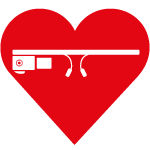
\includegraphics[scale=0.5]{immagini/vhc.png}
        \caption{Logo VisionHealthCare}
        \label{logoVHC}
      \end{figure}

      I Google Glass si interfacciano con un'applicazione installata nello smartphone e si collegano tramite questo ai servizi di OrmaWeb.\\
      Questi occhiali permettono di registrare, durante l'operazione, note vocali correlate da video e foto che sono utili alla documentazione dell'operazione ma anche per attività di ricerca e di insegnamento.\\
      Il sistema permette di automatizzare buona parte di procedure di verbalizzazione dell'intervento, trascrivendo il testo registrato e unendolo ai dati già presenti in OrmaWeb.\\
      Questa soluzione permette di lavorare a mani libere e allo stesso tempo di ricevere dati aggiuntivi sullo stato del paziente.
    \newpage
    \subsubsection*{NapkinForever - Pininfarina Segno}
      Vision Lab Apps collabora anche con NapkinForever, azienda italiana di penne e stilo di design che da poco ha raggiunto un accordo di collaborazione con Pininfarina.\\
      Ha realizzato una presentazione virtuale dell'impresa per il Paperworld 2017, la più grande fiera mondiale di prodotti per l'ufficio e strumenti di scrittura.\\
      Questo progetto consisteva nella simulazione virtuale dei prodotti proposti da NapkinForever, inseriti in scenografie ad hoc, fornendo informazioni su di essi.\\
      Le tecnologie utilizzate comprendevano l'utilizzo di uno smartphone in accoppiata con i Google Cardboard, un apparato di lenti montate su un telaio di cartone.
      L'utilizzo di \textit{hardware} fatto di materiali poveri permetteva di fornire una buona esperienza d'uso ad un prezzo competitivo.
      Attualmente stanno sviluppando il sito web della nuova linea di prodotti nata dalla collaborazione con Pininfarina, design house di fama internazionale.
      \begin{flushleft}
        \begin{figure}[h]
          \centering
          
\includegraphics[scale=0.15]{immagini/forever.png}
          \caption{Logo NapkinForever e del nuovo \textit{brand} in collaborazione con Pininfarina}
          \label{logoNapkin}
        \end{figure}
      \end{flushleft}
  \section{Premi e certificazioni}
    \subsubsection*{UniCredit Start Lab}
    Vision Lab Apps ha partecipato alla competizione tra startup UniCredit Start Lab 2017.
    Durante questo evento le aziende che vi hanno partecipato hanno proposto le loro idee innovative in vari ambiti.\\
    L'azienda è stata valutata e inserita tra le 10 finaliste, guadagnando un periodo di incubazione e accelerazione da parte di UniCredit a partire da Settembre 2017.
    \begin{figure}[h]
      \centering
      
\includegraphics[scale=0.5]{immagini/unicredit.png}
      \caption{Logo di UniCredit Start Lab}
      \label{logoUnicredit}
    \end{figure}
    \newpage
    \subsubsection*{CES 2018 - Consumer Elettronic Show}
      Come conseguenza del periodo di incubazione e accelerazione da parte di UniCredit, Vision Lab Apps ha potuto partecipare, dopo un periodo di selezione, all'evento CES 2018.\\
      Il CES (Consumer Elettronic Show) è la più grande fiera mondiale di tecnologia di consumo e parteciparvi è senza dubbio un trampolino di lancio per avere maggiore visibilità a livello internazionale.\\
      Durante questo evento di quattro giorni tenutosi a Las Vegas, un altro indice di successo è stata la partecipazione dell'azienda all'elevator pitch di TechStars, incubatore di startup famoso a livello internazionale, come una delle 10 migliori realtà presenti all'evento.
      \begin{figure}[h]
        \centering
        
\includegraphics[scale=0.3]{immagini/ces.png}
        \caption{Logo CES - Consumer Elettronic Show}
        \label{logoCes}
      \end{figure}
  \newpage
  \section{Organizzazione aziendale}
    \subsection{Modello di sviluppo}
      Vision Lab Apps lavora con un metodo di sviluppo \textit{Agile} di tipo \textit{Scrum}.\\
      Questo modello si basa su principi fondamentali per svincolarsi da eccessiva rigidità. I principi fondamentali sono:
      \begin{itemize}
        \item le persone e le interazioni sono più importanti rispetto ai processi e agli strumenti;
        \item è molto più importante il \textit{software} rispetto alla documentazione;
        \item è molto più importante rispondere al cambiamento rispetto all'agire secondo un piano.
      \end{itemize}
      Questo pone una minore rigidità sulla documentazione e sulle formalità del prodotto, permettendo le modifiche in corso d'opera e maggiore flessibilità ai cambiamenti.\\
      Il metodo consiste nel fissare dei periodi di tempo brevi, gli \nameref{Sprint}, in cui vengono eseguite delle attività dette \nameref{Task}.\\
      In ogni \nameref{Sprint} il \textit{team} decide che \nameref{Task} eseguire e a chi vengono assegnati, prendendoli da un insieme organizzato detto \textit{backlog} del prodotto. In questo modo viene a crearsi un altro insieme organizzato di \nameref{Task} detto \textit{backlog} dello \nameref{Sprint}.\\
      Ogni giorno il \textit{team} si ritrova per una breve riunione in cui viene controllato lo stato dei vari \nameref{Task} o se sono sorte problematiche nella loro esecuzione, il \textit{daily scrum}.\\
      Al completamento di tutti i \nameref{Task} e quindi alla fine dello \nameref{Sprint} viene fatta un'ulteriore riunione in cui vengono discussi i problemi incontrati nell'esecuzione dei \nameref{Task}, discutendo inoltre quali precauzioni prendere per incorrere nuovamente nelle stesse complicazioni.\\\\
      Trattandosi di un metodo \textit{Agile} la documentazione è molto ridotta e quindi nasce il concetto di user story, documento fondamentale che contiene le richieste del cliente e le decisioni prese con lo stesso durante un incontro faccia a faccia.\\
      La presenza simultanea del cliente e di almeno un membro del \textit{team} permette una maggiore trasparenza e chiarezza riguardo le richieste del consumatore.\\
      Questo favorisce, inoltre, un'implementazione più semplice e diretta degli obiettivi da raggiungere.
      \newpage
      Per coordinamento del lavoro, l'assegnazione dei \nameref{Task} e il controllo dello stato degli stessi, l'azienda utilizza un applicazione web, Kanboard, che permette la creazione dei \nameref{Task}, la sua assegnazione con scadenze e le priorità.
      Tutto questa in una grafica che dà l'idea di una lavagna con dei post-it che possono essere spostati in base allo stato del \nameref{Task}.
      \begin{figure}[h]
        \centering
        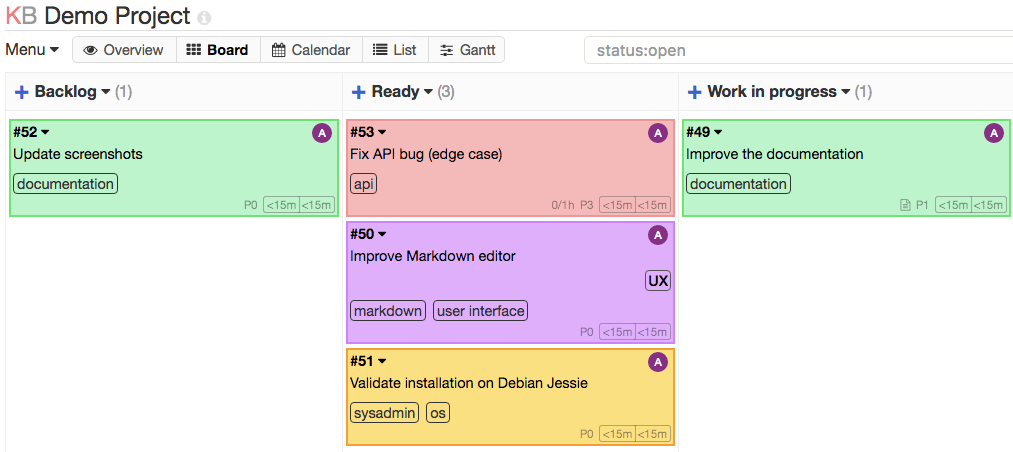
\includegraphics[scale=0.3]{immagini/board.png}
        \caption{Esempio della grafica di Kanboard}
        \label{kan}
      \end{figure}\\
      Questa applicazione web, visualizzabile da tutti i membri del \textit{team}, permette di avere una visione comune.\\
      Inoltre permette al \nameref{PM} di comprende le tempistiche di sviluppo per eventualmente capire come verrebbe gestita, a livello temporale, l'aggiunta di nuovi \nameref{Task} fornendo cioè una visione generale dell'utilizzo delle risorse.
    \subsection{Comunicazione}
      Per comunicare i membri del \textit{team} usano Slack, uno strumento di collaborazione aziendale che permette di inviare messaggi in modo istantaneo ai membri del \textit{team}.\\
      Inoltre viene usato anche Google Hangouts e Skype per permettere comunicazioni a distanza nel caso non fosse possibile riunire tutti i membri del \textit{team} nello stesso posto.
  \section{Tecnologie utilizzate dall'azienda}
    \subsection{Firebase}
      Firebase è una piattaforma di sviluppo per applicazioni web e \textit{mobile}, parte di Google Cloud Platform; fornisce servizi di scambio messaggi e basi di dati in tempo reale, spazio di archiviazione, sistemi di autenticazione, web \textit{hosting} e \textit{test} automatici per applicazioni Android.\\
      La piattaforma fornisce anche un servizio di analisi e profilazione degli utenti ed è presente anche l'integrazione con il sistema di annunci pubblicitari di Google.
      \begin{figure}[h]
        \centering
        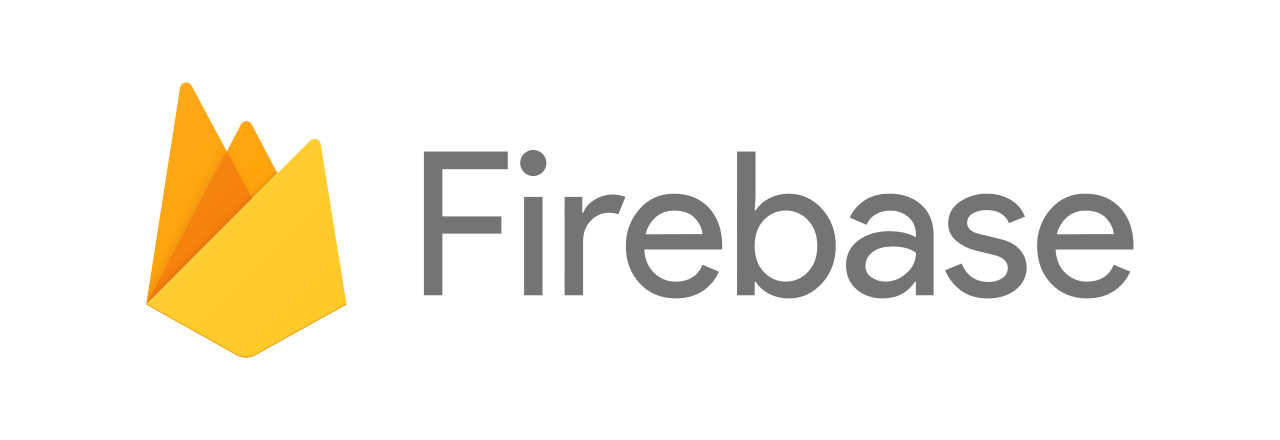
\includegraphics[scale=0.2]{immagini/firebase.png}
        \caption{Logo Firebase}
        \label{logoFire}
      \end{figure}
    \subsection{Java}
      \nameref{Java} è un linguaggio di programmazione ad alto livello orientato agli oggetti ed è stato pensato e progettato per essere indipendente dalla piattaforma in cui viene eseguito.
      Supera questo ostacolo eseguendo i programmi su una macchina virtuale, la \nameref{JVM}, in modo che non venga considerato importante il sistema sottostante.\\
      Infatti il codice compilato che viene eseguito su una piattaforma non deve essere ricompilato per essere eseguito su una piattaforma diversa. Questo grazie al fatto che il prodotto della compilazione è nel formato detto bytecode che può essere riutilizzato da qualsiasi implementazione della \nameref{JVM}.\\
      Viene utilizzato per lo sviluppo di applicazioni su dispositivi \textit{mobile} ma anche nel caso di servizi web che necessitano di avere un alto parallelismo e concorrenza.
      \begin{figure}[h]
        \centering
        
\includegraphics[scale=0.12]{immagini/java.png}
        \caption{Logo Java}
        \label{java}
      \end{figure}
    \newpage
    \subsection{Android}
      Android è un sistema operativo fortemente basato su \nameref{Java} e viene utilizzato appunto per lo sviluppo di applicazioni per dispositivi \textit{mobile}.\\
      Consiste in una versione minima del \textit{kernel} Linux, in cui sono presenti i driver specializzati dell'\textit{hardware} del dispositivo.\\
      Sopra ad esso è presente un layer che permette di astrarre l'\textit{hardware} e permette di farlo comunicare appunto con gli strati superiori.\\
      Il layer superiore è composto da librerie native in C o C++ e dall'equivalente della \nameref{JVM} in \nameref{Java}, il \textit{runtime} Android, che però è specializzato nell'esecuzione su dispositivi \textit{mobile}.\\
      Infine gli strati superiori sono un'\nameref{API} per l'accesso alle risorse del sistema e le applicazioni.
      \begin{figure}[h]
        \centering
        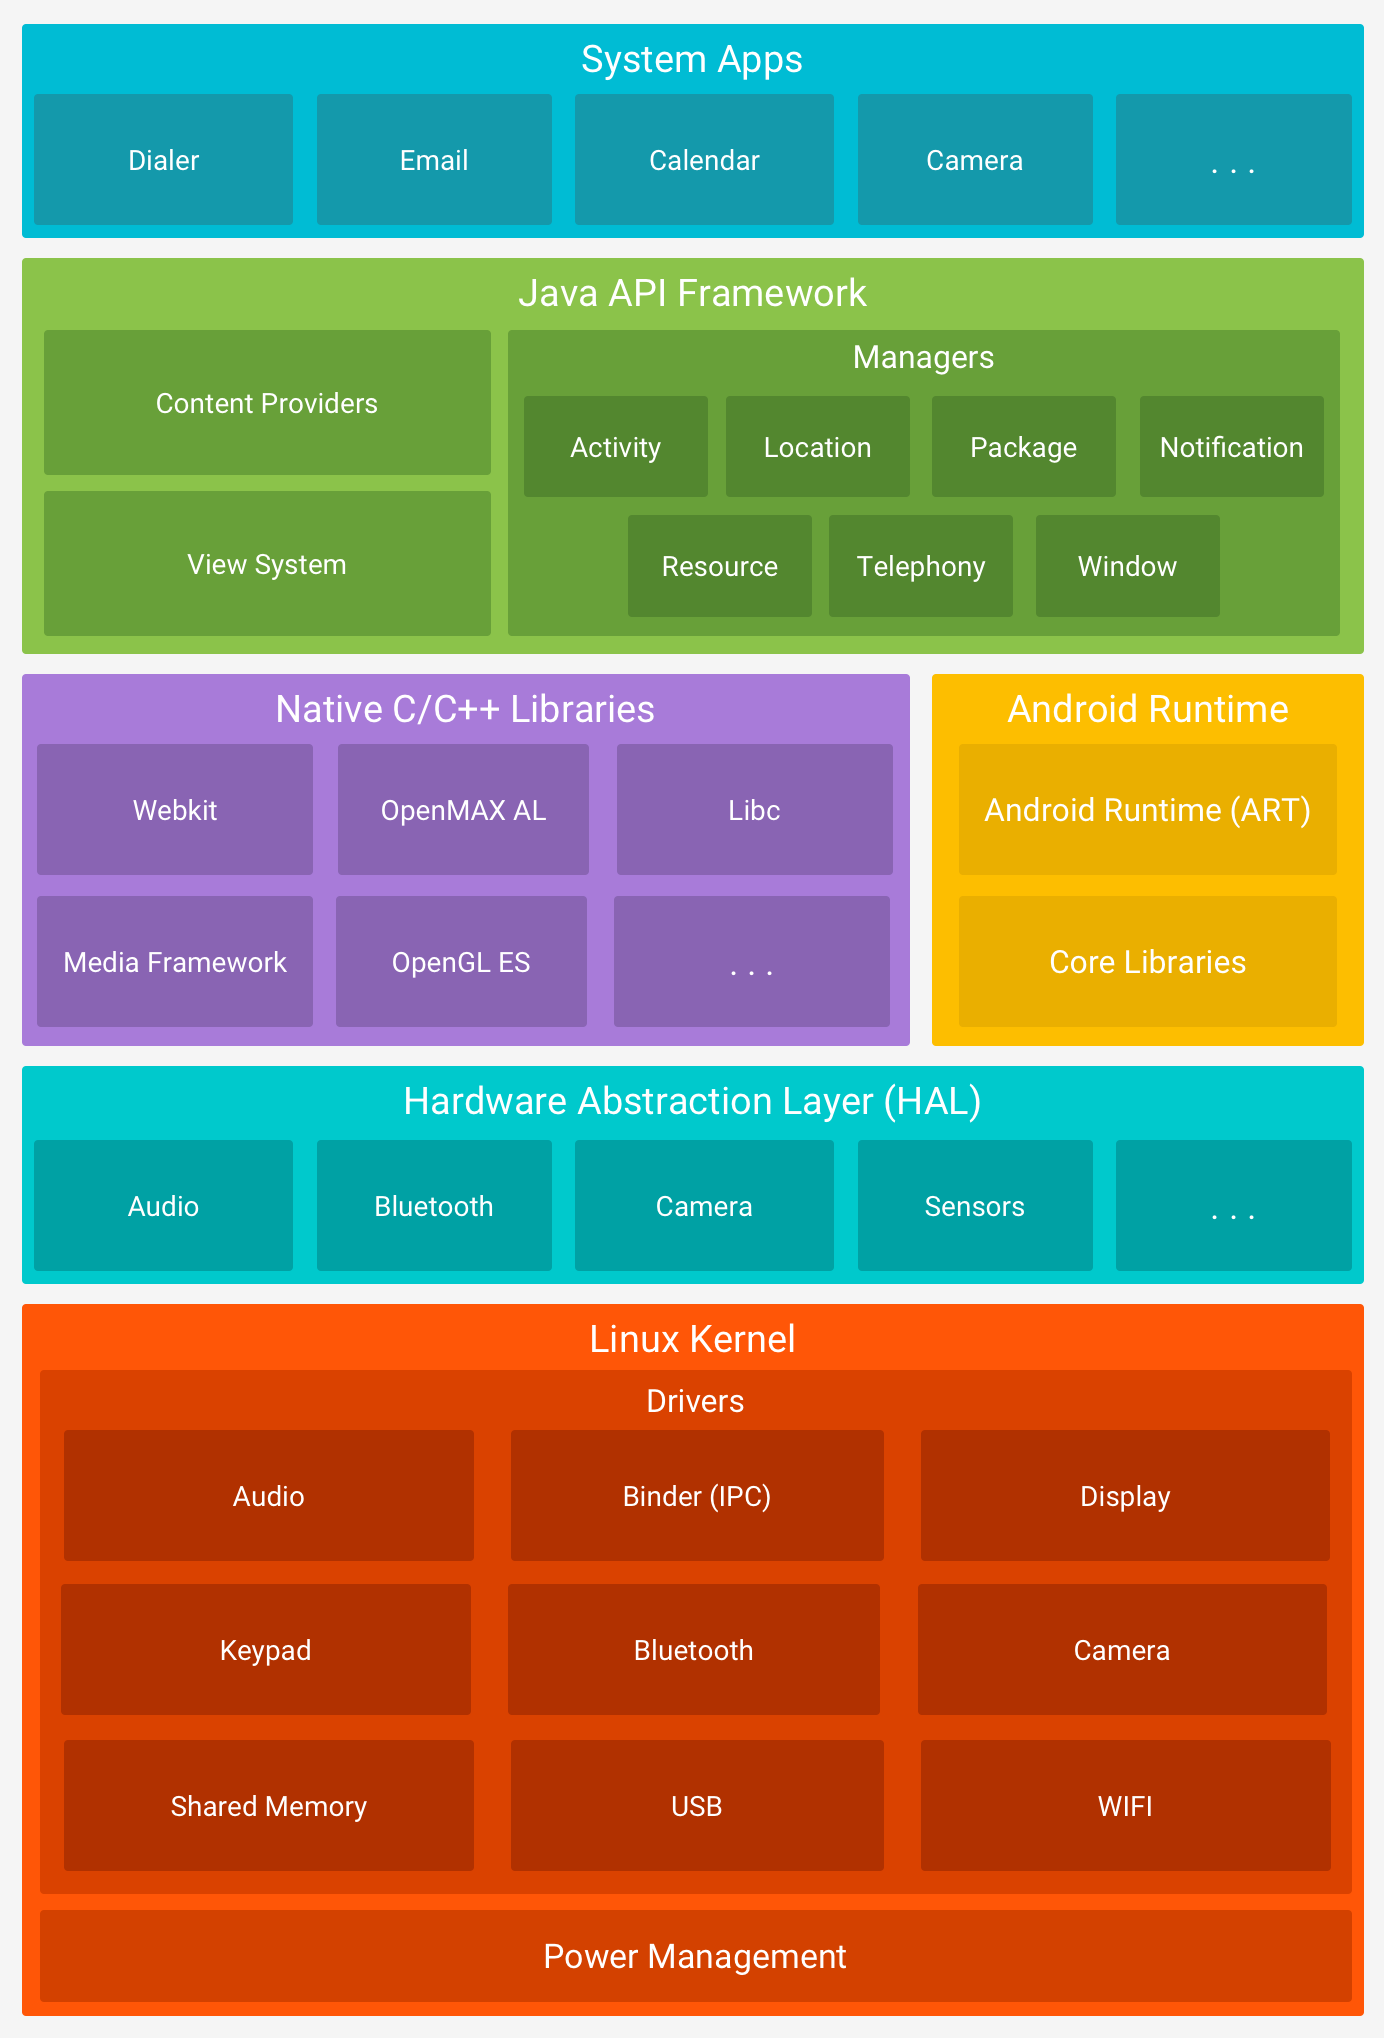
\includegraphics[scale=0.11]{immagini/android.png}
        \caption{Architettura di Android}
        \label{android}
      \end{figure}
    \newpage
    \subsection{Git e Bitbucket}
      Come \textit{software} di controllo di versione distribuito viene utilizzato Git.\\
      Attraverso l'utilizzo di Git è possibile gestire progetti anche molto complessi in modo efficiente, infatti perché consente a due o più persone di lavorare contemporaneamente sullo stesso file, senza perdita di consistenza, senza la necessità di collegamento di rete e senza conservare copie di backup in luoghi separati.\\
      L'azienda ha deciso di sfruttare, come \textit{hosting} per le proprie \textit{repository}, BitBucket in modo da facilitare la gestione del codice ed automatizzare alcune procedure.\\
      Infatti BitBucket integra il concetto di \textit{pipeline}, cioè una sequenza di \nameref{Task} che permette di eseguire script. In questo modo è possibile automatizzare i \textit{test} che verranno eseguiti ad ogni \textit{commit}.
      \begin{figure}[h]
        \centering
        
\includegraphics[scale=0.3]{immagini/bitbucket.png}
        \caption{Logo Bitbucket}
        \label{bit}
      \end{figure}
    \subsection{G Suite}
      È la soluzione per l'ufficio di Google e offre una gestione completa di email, \textit{editor} di testo, fogli di calcolo, calendario e archivio.\\
      Il principale vantaggio nell'utilizzarla è la possibilità di accedere ai dati in completa mobilità.\\
      I prodotti più utilizzati sono Drive per lo \textit{storage}, Docs per i documenti, Spreadsheet per i fogli di calcolo, Gmail per la gestione delle email. Include inoltre Hangouts che, come detto precedentemente viene utilizzato per le comunicazioni.
      \begin{figure}[h]
        \centering
        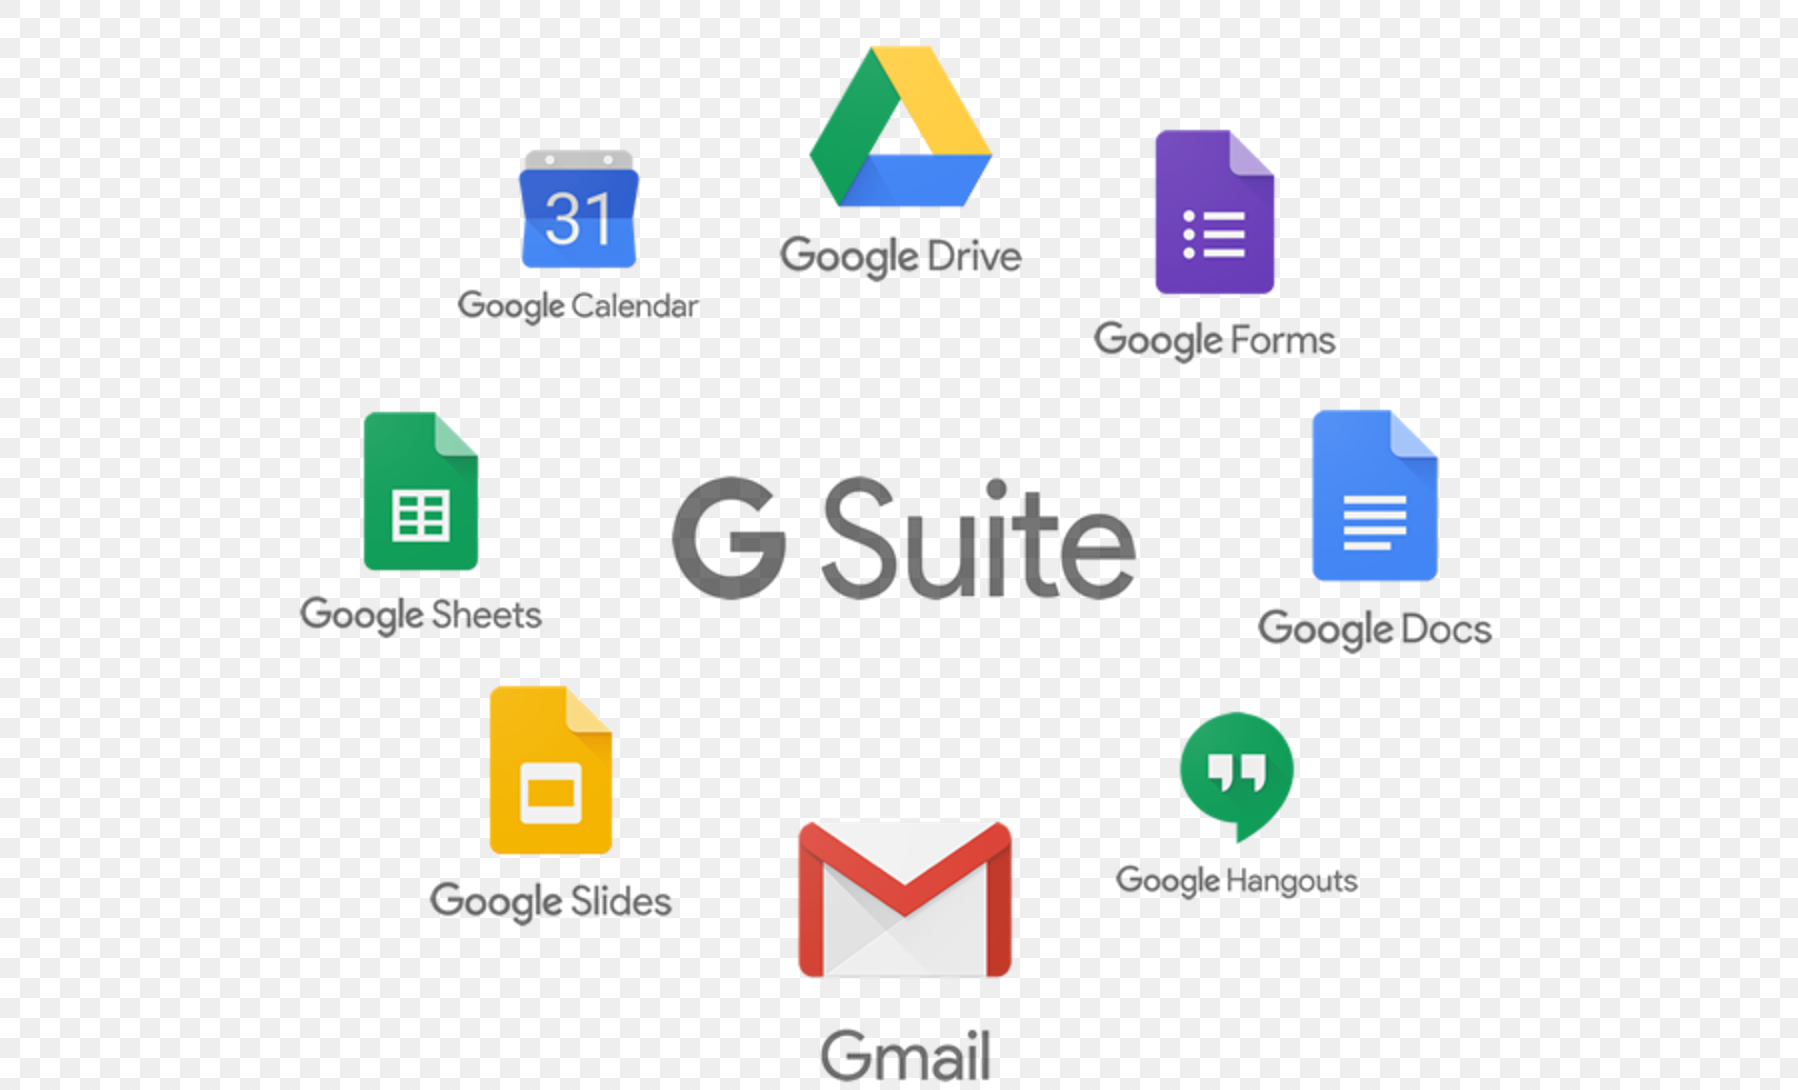
\includegraphics[scale=0.2]{immagini/gsuite.png}
        \caption{Logo G suite con alcuni prodotti}
        \label{logog}
      \end{figure}
      \newpage
      \null
      \thispagestyle{empty}
      \newpage
